\documentclass[a4paper, 12pt]{article}
\usepackage[utf8]{inputenc}
\usepackage[left=2cm, top=3cm, text={17cm, 24cm}]{geometry}
\usepackage[IL2]{fontenc}
\usepackage[slovak]{babel}
\usepackage{times}
\usepackage{mathtools}
\usepackage{epic}
\usepackage{amssymb}
\usepackage{amsthm}
\usepackage{graphics}
\usepackage[unicode]{hyperref}
\usepackage{ dsfont }
\usepackage{comment}
\usepackage{placeins}
\usepackage{float}
\hypersetup{colorlinks = false, hypertexnames = false}
\renewcommand*\rmdefault{ptm}

\begin{document}

\begin{titlepage}
\begin{center}
\thispagestyle{empty}
{\Huge
\textsc{Vysoké učení technické v Brně\\}}
{\LARGE
\textsc {Fakulta informačních technologií\\[0.4em]}}

\vspace{\stretch{0.4}}

{\LARGE Dokumentácia k projektu: \\[0.3em]}
{\LARGE Implementácia prekladača imperatívneho jazyka IFJ21}
{\LARGE \\Tím 117, varianta I\\[0.3em]}
\vspace{\stretch{0.6}}
{\Large 
Jiřina Frýbortová (xfrybo01) = $\infty$\,\%  \\ 
Jana Kováčiková (xkovac59) = $\infty$\,\%  \\ 
Alexander Rastislav Okrucký (xokruc00) = $\infty$\,\%  \\ 
Patrik Skaloš (xskalo01) = $\infty$\,\% - vedúci tímu\\}
\end{center}

\end{titlepage}

\section{Rozdelenie práce}
Už od začiatku sme sa snažili na všetkom pracovať spolu. Naša práca začala pri spoločnom návrhu konečného automatu a celý skener sme tiež naprogramovali spoločne. Veľmi nám to pomohlo presne pochopiť, čo a ako je potrebujeme urobiť. Sme tiež presvedčení, že nám to pomohlo napísať menej chybový kód.

Ďalším krokom bola implementácia binárneho stromu - tu sa naša práca rozdelila a nepracovali sme na ňom všetci. Z binárneho stromu sme ďalej naprogramovali zásobník stromov - tabuľku symbolov. Parser bola jedna z najzložitejších častí a tak sme znovu zvolili spoločnú prácu - od návrhu gramatiky až po samotnú implementáciu a testovanie. Precedenčnú analýzu sme začali najprv robiť spolu, no z časových dôvodov ju mal nakoniec na starosti vedúci nášho tímu - Patrik Skaloš. Generátor mal na starosti Alexander Okrucký, no každý sme prispeli svojou časťou.\\

\noindent\textbf{Rozdelenie práce na ktorej sme nerobili spoločne:\\}

\noindent Jiřina Frýbortová - binárny strom, dokumentácia
\\Jana Kováčiková - binárny strom, dokumentácia, prekreslenie konečného automatu do finálnej podoby
\\Alexander Rastislav Okrucký - generátor cieľového kódu, testy
\\Patrik Skaloš - tabulka symbolov, precedenčná analýza, makefile, testy\\

\noindent Vyššie spomenuté časti projektu sme síce mali rozdelené, no navzájom sme si aj napriek tomu pomáhali a intenzívne o problémoch aj riešeniach komunikovali.

\section{Organizácia}
Dá sa povedať, že najdôležitejší bol verzovací nástroj Git. Súbory sme v ňom mali rozdelené do vetí podľa celkov, tak aby sa na nich dalo pracovať paralelne a nevznikali konflikty. Zároveň sme v ňom mali históri všetkých súborov a tak sme sa kedykoľvek vedeli vrátiť k pôvodnej verzii.

Na komunikáciu sme využívali aplikáciu Discord v ktorej sme si vytvorili kanály na bežné písanie, termíny ale aj hlasový kanál na naše meetingy. Výhodou bola určite možnosť pripnutia správ aby sme mali dôležité veci vždy po ruke a nemuseli ich pracne hľadať v histórii konverzácie. 

Ďalšou veľmi dôležitou aplikáciou bola Trello (to-do list). Vytvorili sme si stĺpce, ktoré značili či už je daná úloha hotová, pracuje sa na nej alebo je potrebné ju otestovať. Do stĺpcov sme následne pridávali úlohy a priebežne sme tento zoznam aktualizovali. K jednotlivým úlohám sa dali taktiež písať podúlohy, čo určite pomohlo v prehľadnosti a efektivite práce.

\section{Realizácia}

Syntaxou riadený preklad sme realizovali pomocou jednoprechodovej analýzy zdrojového kódu. Náš program nevytvára medzikód ale priamo generuje cieľový kód v jazyku IFJcode21. V prípade nájdenia chyby sa preklad kódu ihneď a bez zotavenia ukončí, na štandardný chybový výstup vypíšeme chybovú hlášku a približné číslo riadku, na ktorom k chybe došlo.

\subsection{Lexikální analýza}

\subsubsection{Návrh konečného automatu}

Počiatočný stav automatu, je kruh S. Šípky v konečnom automate značia, aký znak (množina znakov) je potrebný na prechod z predchádzajúceho do nového stavu. Končený stav v automate značíme hrubším zvýraznením namiesto dvoch kruhov.

\begin{center}
    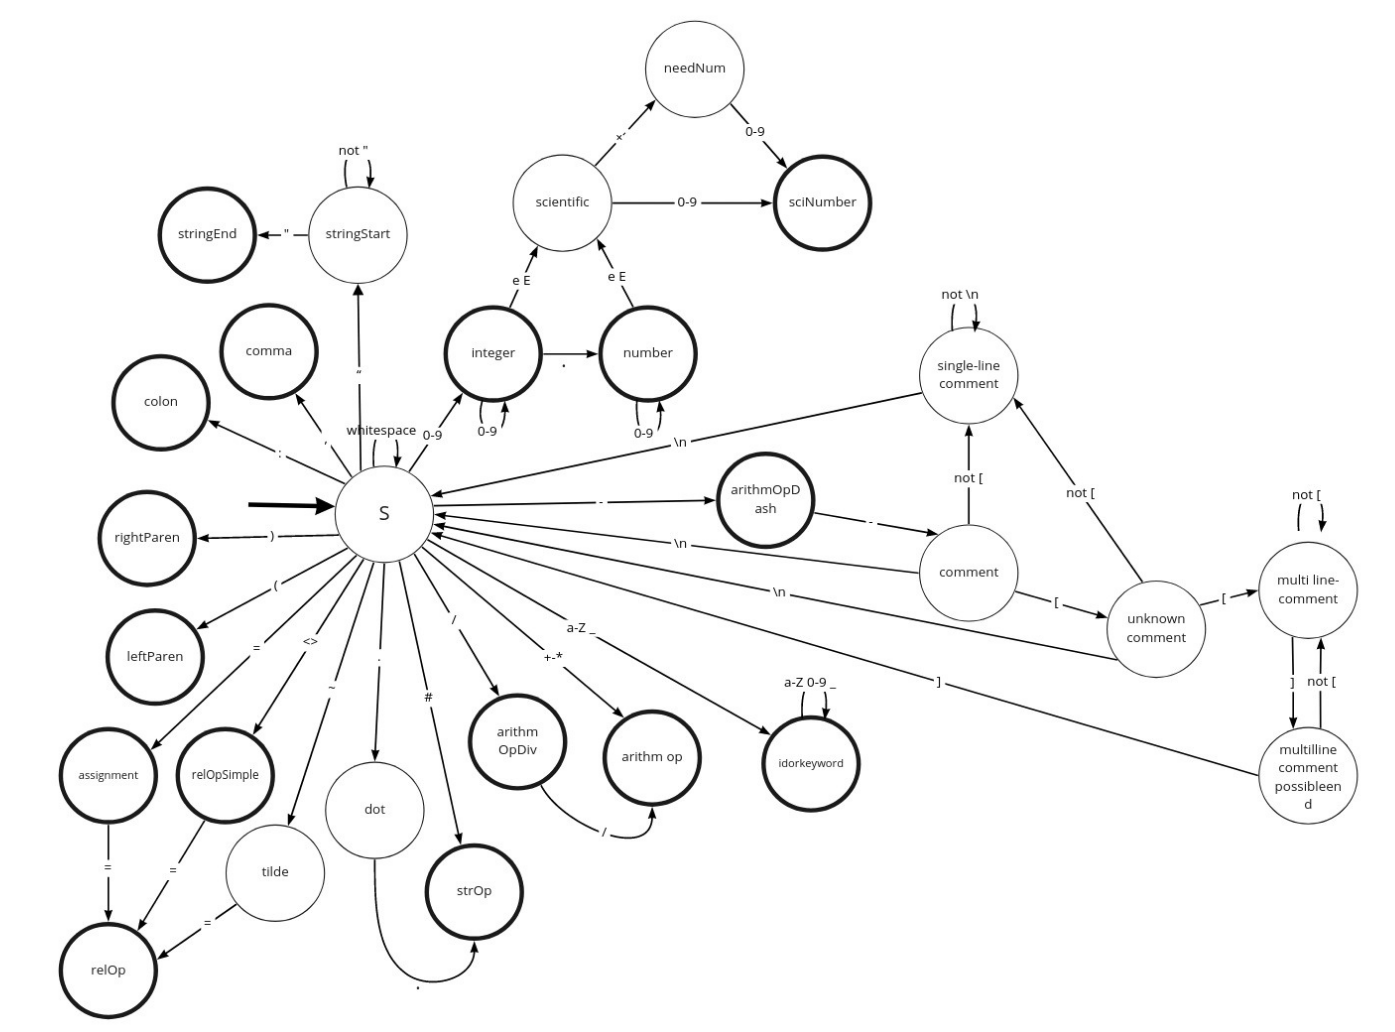
\includegraphics[scale=0.49]{fsm.png}
\end{center}

Graf konečného automatu nájdete taktiež v prílohách, kde sa náchadza vo väčšom rozlíšení.


\subsubsection{Skener}
Podľa návrhu konečného automatu sme realizovali implementáciu skeneru. Skener náčítava postupne znaky až kým nenačíta celý token ktorý predá parseru. Ak pri načítaní skener načíta o znak viac, vrátime ho na stdin. Scanner umožnuje funkciu stash, čo znamená že token vieme vrátiť.

Niektoré stavy, ktoré sú konečné a nedá sa z nich prejsť do iného stavu v skaneri neimplementujeme a na miesto prechodu do týchto stavov vrátime aktuálny token.

V prípade EOF vraciame prázdny token a komentáre aj biele znaky sú ignorované (sú samozrejme zaznamenané ako oddelenie tokenov).

Keď skener narazí na chybu, vráti parseru adekvátny chybový kód (podľa nájdenéj chyby lexikálny alebo interný) a prázdny token.

V skeneri neriešime, či sa jedná o identifikátor alebo kľúčové slovo\,--\,považujeme ich za rovnaký typ tokenu. Dá sa povedať, že so skeneru vraciame len tieto typy tokenov: meno (identifikátor, kľúčové slovo), literál, operátor a špeciálne znaky (čiarka, dvojbodka).

Samotná implementácia skeneru je nasledovná:
Po zavolaní funkcia scanner() číta znaky zo štandardného vstupu a podľa pravidiel konečného automatu a aktuálneho znaku mení stavy. Pri načítaní zakázaného znaku vráti chybu, pri neočakávanom znaku (ak neexistuje pravidlo na prechod) tento znak vráti na štandardný vstup a vráti token volajúcej funkcii. Štruktúra tokenu obsahuje informáciu o type tokenu a jeho obsahu (meno identifikátoru, literál, ...).

\subsubsection{Tabuľka symbolov}

Tabuľku symbolov sme implementovali pomocou binárneho vyhľadávacieho stromu, čo však nestačilo. Vo výsledku ju tvorí zásobník binárnych vyhľadávacích stromov (ďalej BST)\,--\,každý prvok zásobníku obsahuje ukazateľ na jeden BST (jeho koreň), hĺbku zanorenia BST a ukazateľ na nasledujúci prvok. Každý prvok BST klasicky obsahuje kľúč, ukazatele na ľavý a pravý prvok a dáta. Štruktúra pre tieto dáta obsahuje:
\begin{itemize}
    \item \textbf{string}: meno identifikátoru vo vygenerovanom kóde
    \item \textbf{bool}: značí či je identifikátor premennou alebo funkciou
    \item Dáta dôležité, ak je identifikátor \textbf{premennou}:
    \begin{itemize}
        \item \textbf{integer}: enumerácia dátového typu
    \end{itemize}
    \item Dáta dôležité, ak je identifikátor \textbf{funkciou}:
    \begin{itemize}
        \item \textbf{bool}: značí, či bola funkcia deklarovaná
        \item \textbf{bool}: značí, či bola funkcia definovaná
        \item \textbf{pole typu integer}: enumerácie dátových typov parametrov
        \item \textbf{pole typu string}: mená parametrov
        \item \textbf{pole typu integer}: enumerácie dátových typov návratových hodnôt
    \end{itemize}
\end{itemize}
Nad tabuľkou symbolov máme implementované tieto operácie:
\begin{itemize}
    \item \textbf{STInit}: inicializácia
    \item \textbf{STPush}: pridanie nového (prázdneho) BST na vrchol zásobníku
    \item \textbf{STPop}: odstránenie BST z vrcholu zásobníku
    \item \textbf{STInsert}: vloženie nového prvku do BST na vrchole zásobníku\,--\,dáta sú inicializované na nepovolené hodnoty
    \item \textbf{STFind}: vráti prvok BST so zhodným vyhľadávacím kľúčom
    \item Pre nasledujúce operácie sú implementované dve funkcie\,--\,na nastavenie (\textbf{STSet}) a čítanie (\textbf{STGet}):
    \begin{itemize}
        \item \textbf{IsVariable}: pravdivostná hodnota, či je identifikátor premennou (ak nie je pravda, je funkciou)
        \item \textbf{VarDataType}: dátový typ premennej
        \item \textbf{FnDefined}: pravdivostná hodnota, či bola funkcia definovaná
        \item \textbf{FnDeclared}: pravdivostná hodnota, či bola funkcia deklarovaná
        \item \textbf{Name}: meno identifikátora v generovanom kóde
    \end{itemize}
    \item Pre nasledujúce operácie s nafukovacími poľami sú taktiež dve funkcie\,--\,na pridanie na koniec poľa (\textbf{STAppend}) a čítanie (\textbf{STGet}) z poľa:
    \begin{itemize}
        \item \textbf{ParamType}: dátový typ parametra funkcie
        \item \textbf{ParamName}: meno parametra funkcie
        \item \textbf{RetType}: dátový typ návratovej hodnoty funkcie
    \end{itemize}
    \item \textbf{STGetDepth}: vráti číslo reprezentujúce zanorenie BST na vrchole zásobníku
    \item \textbf{STFindUndefinedFunctions}: hľadá, či je v BST na vrchole zásobníku funkcia, ktorá bola deklarovaná ale nebola definovaná
    
    
\end{itemize}

\subsection{Syntaktická analýza}

\subsubsection{LL tabuľka}

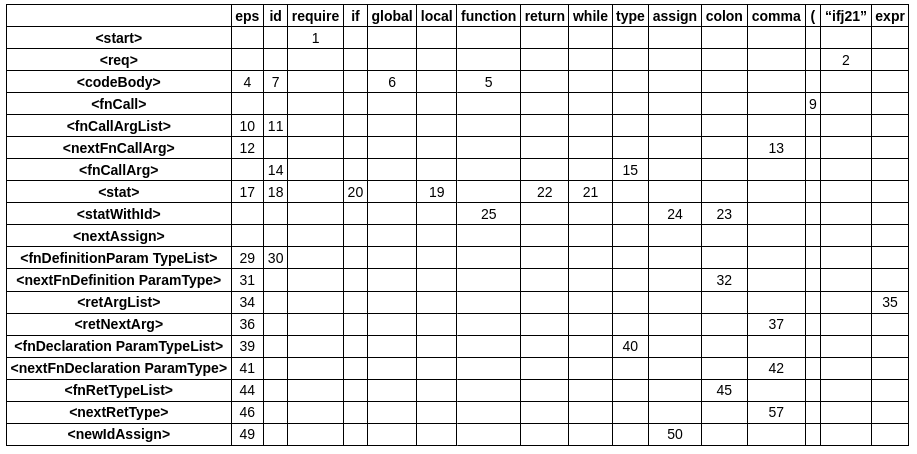
\includegraphics[scale=0.55]{ll_table.png}

\subsubsection{Bezkontextová gramatika}

\begin{tabbing}
42. \textless nextFnDeclarationParamType\textgreater \; \= \textrightarrow \quad \= \kill

\noindent 01. \textless start\textgreater                      \> \textrightarrow \>  require \textless req\textgreater \textless codeBody\textgreater \\
02. \textless req\textgreater                        \> \textrightarrow \>   ``ifj21"  \\\\

\noindent 04. \textless codeBody\textgreater                   \> \textrightarrow \>  eps \\
05. \textless codeBody\textgreater                   \> \textrightarrow \>  function [id] ( \textless fnDefinitionParamTypeList\textgreater ) \\ \> \> \textless fnRetTypeList\textgreater \textless stat\textgreater end \textless codeBody\textgreater \\
06. \textless codeBody\textgreater                   \> \textrightarrow \>  global [id] : function ( \textless fnDeclarationParamTypeList\textgreater )\\ \> \> \textless fnRetTypeList\textgreater \textless codeBody\textgreater \\
07. \textless codeBody\textgreater                   \> \textrightarrow \>  [id] \textless fnCall\textgreater \textless codeBody\textgreater \\ \\

\noindent 09. \textless fnCall\textgreater                     \> \textrightarrow \>  ( \textless fnCallArgList\textgreater ) \\
10. \textless fnCallArgList\textgreater              \> \textrightarrow \>  eps \\
11. \textless fnCallArgList\textgreater              \> \textrightarrow \>  \textless fnCallArg\textgreater \textless nextFnCallArg\textgreater \\
12. \textless nextFnCallArg\textgreater              \> \textrightarrow \>  eps \\
13. \textless nextFnCallArg\textgreater              \> \textrightarrow \>  , \textless fnCallArg\textgreater \textless nextFnCallArg\textgreater \\
14. \textless fnCallArg\textgreater                  \> \textrightarrow \>  [id] \\
15. \textless fnCallArg\textgreater                  \> \textrightarrow \>  [literal] \\ \\

\noindent 17. \textless stat\textgreater                       \> \textrightarrow \>  eps \\
18. \textless stat\textgreater                       \> \textrightarrow \>  [id] \textless statWithId\textgreater \textless stat\textgreater \\
19. \textless stat\textgreater                       \> \textrightarrow \>  local [id] : [type] \textless newIdAssign\textgreater \textless stat\textgreater \\
20. \textless stat\textgreater                       \> \textrightarrow \>  if \textless expr\textgreater then \textless stat\textgreater else \textless stat\textgreater end \textless stat\textgreater \\
21. \textless stat\textgreater                       \> \textrightarrow \>  while \textless expr\textgreater do \textless stat\textgreater end \textless stat\textgreater \\
22. \textless stat\textgreater                       \> \textrightarrow \>  return \textless retArgList\textgreater \textless stat\textgreater  \\
23. \textless statWithId\textgreater                 \> \textrightarrow \>  , [id] \textless nextAssign\textgreater \textless expr\textgreater \\
24. \textless statWithId\textgreater                 \> \textrightarrow \>  = \textless expr\textgreater \\
25. \textless statWithId\textgreater                 \> \textrightarrow \>  \textless fnCall\textgreater \\
26. \textless nextAssign\textgreater                 \> \textrightarrow \>  , [id] \textless nextAssign\textgreater \textless expr\textgreater\\
27. \textless nextAssign\textgreater                 \> \textrightarrow \>  = \\ \\

\noindent 29. \textless fnDefinitionParamTypeList\textgreater  \> \textrightarrow \>  eps \\
30. \textless fnDefinitionParamTypeList\textgreater  \> \textrightarrow \>  [id] : [type] \textless nextFnDefinitionParamType\textgreater \\
31. \textless nextFnDefinitionParamType\textgreater  \> \textrightarrow \>  eps \\
32. \textless nextFnDefinitionParamType\textgreater  \> \textrightarrow \>  , [id] : [type] \textless nextFnDefinitionParamType\textgreater \\ \\

\noindent 34. \textless retArgList\textgreater                 \> \textrightarrow \>  eps \\
35. \textless retArgList\textgreater                 \> \textrightarrow \>  \textless expr\textgreater \textless retNextArg\textgreater \\
36. \textless retNextArg\textgreater                 \> \textrightarrow \>  eps \\
37. \textless retNextArg\textgreater                 \> \textrightarrow \>  , \textless expr\textgreater \textless retNextArg\textgreater \\ \\

\noindent 39. \textless fnDeclarationParamTypeList\textgreater \> \textrightarrow \>  eps \\
40. \textless fnDeclarationParamTypeList\textgreater \> \textrightarrow \>  [type] \textless nextFnDeclarationParamType\textgreater \\
41. \textless nextFnDeclarationParamType\textgreater \> \textrightarrow \>  eps \\
42. \textless nextFnDeclarationParamType\textgreater \> \textrightarrow \>  , [type] \textless nextFnDeclarationParamType\textgreater \\ \\

\noindent 44. \textless fnRetTypeList\textgreater              \> \textrightarrow \>  eps  \\
45. \textless fnRetTypeList\textgreater              \> \textrightarrow \>  : [type] \textless nextRetType\textgreater \\
46. \textless nextRetType\textgreater                \> \textrightarrow \>  eps \\
47. \textless nextRetType\textgreater                \> \textrightarrow \>  , [type] \textless nextRetType\textgreater \\

\noindent 49. \textless newIdAssign\textgreater                \> \textrightarrow \>  eps \\
50. \textless newIdAssign\textgreater                \> \textrightarrow \>  = \textless expr\textgreater \\ \\  
\end{tabbing}


\subsubsection{Precedenčná tabuľka}
\FloatBarrier
\begin{table}[!ht]
\begin{tabular}{|c|c|c|c|c|c|c|c|c|c|c|c|c|c|c|c|c|c|}
\hline
                         & \textbf{\#}    & \textbf{*}     & \textbf{/}     & \textbf{//}    & \textbf{+}     & \textbf{-}     & \textbf{..}    & \textbf{\textless{}} & \textbf{\textless{}=} & \textbf{\textgreater{}} & \textbf{\textgreater{}=} & \textbf{==}    & \textbf{$\sim$=} & \textbf{(}  & \textbf{)}     & \textbf{id} & \textbf{\$}    \\ \hline
\textbf{\#}              &                & \textgreater{} & \textgreater{} & \textgreater{} & \textgreater{} & \textgreater{} & \textgreater{} & \textgreater{}       & \textgreater{}        & \textgreater{}          & \textgreater{}           & \textgreater{} & \textgreater{}   & \textless{} & \textgreater{} & \textless{} & \textgreater{} \\ \hline
\textbf{*}               & \textless{}    & \textgreater{} & \textgreater{} & \textgreater{} & \textgreater{} & \textgreater{} & \textgreater{} & \textgreater{}       & \textgreater{}        & \textgreater{}          & \textgreater{}           & \textgreater{} & \textgreater{}   & \textless{} & \textgreater{} & \textless{} & \textgreater{} \\ \hline
\textbf{/}               & \textless{}    & \textgreater{} & \textgreater{} & \textgreater{} & \textgreater{} & \textgreater{} & \textgreater{} & \textgreater{}       & \textgreater{}        & \textgreater{}          & \textgreater{}           & \textgreater{} & \textgreater{}   & \textless{} & \textgreater{} & \textless{} & \textgreater{} \\ \hline
\textbf{//}              & \textless{}    & \textgreater{} & \textgreater{} & \textgreater{} & \textgreater{} & \textgreater{} & \textgreater{} & \textgreater{}       & \textgreater{}        & \textgreater{}          & \textgreater{}           & \textgreater{} & \textgreater{}   & \textless{} & \textgreater{} & \textless{} & \textgreater{} \\ \hline
\textbf{+}               & \textless{}    & \textless{}    & \textless{}    & \textless{}    & \textgreater{} & \textgreater{} & \textgreater{} & \textgreater{}       & \textgreater{}        & \textgreater{}          & \textgreater{}           & \textgreater{} & \textgreater{}   & \textless{} & \textgreater{} & \textless{} & \textgreater{} \\ \hline
\textbf{-}               & \textless{}    & \textless{}    & \textless{}    & \textless{}    & \textgreater{} & \textgreater{} & \textgreater{} & \textgreater{}       & \textgreater{}        & \textgreater{}          & \textgreater{}           & \textgreater{} & \textgreater{}   & \textless{} & \textgreater{} & \textless{} & \textgreater{} \\ \hline
\textbf{..}              & \textless{}    & \textless{}    & \textless{}    & \textless{}    & \textless{}    & \textless{}    & \textless{}    & \textgreater{}       & \textgreater{}        & \textgreater{}          & \textgreater{}           & \textgreater{} & \textgreater{}   & \textless{} & \textgreater{} & \textless{} & \textgreater{} \\ \hline
\textbf{\textless{}}     & \textless{}    & \textless{}    & \textless{}    & \textless{}    & \textless{}    & \textless{}    & \textless{}    & \textgreater{}       & \textgreater{}        & \textgreater{}          & \textgreater{}           & \textgreater{} & \textgreater{}   & \textless{} & \textgreater{} & \textless{} & \textgreater{} \\ \hline
\textbf{\textless{}=}    & \textless{}    & \textless{}    & \textless{}    & \textless{}    & \textless{}    & \textless{}    & \textless{}    & \textgreater{}       & \textgreater{}        & \textgreater{}          & \textgreater{}           & \textgreater{} & \textgreater{}   & \textless{} & \textgreater{} & \textless{} & \textgreater{} \\ \hline
\textbf{\textgreater{}}  & \textless{}    & \textless{}    & \textless{}    & \textless{}    & \textless{}    & \textless{}    & \textless{}    & \textgreater{}       & \textgreater{}        & \textgreater{}          & \textgreater{}           & \textgreater{} & \textgreater{}   & \textless{} & \textgreater{} & \textless{} & \textgreater{} \\ \hline
\textbf{\textgreater{}=} & \textless{}    & \textless{}    & \textless{}    & \textless{}    & \textless{}    & \textless{}    & \textless{}    & \textgreater{}       & \textgreater{}        & \textgreater{}          & \textgreater{}           & \textgreater{} & \textgreater{}   & \textless{} & \textgreater{} & \textless{} & \textgreater{} \\ \hline
\textbf{==}              & \textless{}    & \textless{}    & \textless{}    & \textless{}    & \textless{}    & \textless{}    & \textless{}    & \textgreater{}       & \textgreater{}        & \textgreater{}          & \textgreater{}           & \textgreater{} & \textgreater{}   & \textless{} & \textgreater{} & \textless{} & \textgreater{} \\ \hline
\textbf{$\sim$=}         & \textless{}    & \textless{}    & \textless{}    & \textless{}    & \textless{}    & \textless{}    & \textless{}    & \textgreater{}       & \textgreater{}        & \textgreater{}          & \textgreater{}           & \textgreater{} & \textgreater{}   & \textless{} & \textgreater{} & \textless{} & \textgreater{} \\ \hline
\textbf{(}               & \textless{}    & \textless{}    & \textless{}    & \textless{}    & \textless{}    & \textless{}    & \textless{}    & \textless{}          & \textless{}           & \textless{}             & \textless{}              & \textless{}    & \textless{}      & \textless{} & =              & \textless{} &                \\ \hline
\textbf{)}               & \textgreater{} & \textgreater{} & \textgreater{} & \textgreater{} & \textgreater{} & \textgreater{} & \textgreater{} & \textgreater{}       & \textgreater{}        & \textgreater{}          & \textgreater{}           & \textgreater{} & \textgreater{}   &             & \textgreater{} &             & \textgreater{} \\ \hline
\textbf{id}              & \textgreater{} & \textgreater{} & \textgreater{} & \textgreater{} & \textgreater{} & \textgreater{} & \textgreater{} & \textgreater{}       & \textgreater{}        & \textgreater{}          & \textgreater{}           & \textgreater{} & \textgreater{}   &             & \textgreater{} &             & \textgreater{} \\ \hline
\textbf{\$}              & \textless{}    & \textless{}    & \textless{}    & \textless{}    & \textless{}    & \textless{}    & \textless{}    & \textless{}          & \textless{}           & \textless{}             & \textless{}              & \textless{}    & \textless{}      & \textless{} &                & \textless{} &                \\ \hline
\end{tabular}
\end{table}
\FloatBarrier

\subsubsection{Parser}

Pri parseri sme zvolili rekurzívny zostup. Pri spracovaní výrazu voláme precedenčnú analýzu.

Redefiníciu premenných riešime tak, že sa všetky definície ukladajú do bufferu a ak sa tam už raz daná funkcia nachádza, neuloží sa znovu. Premenné deklarujeme až na konci funkcie. Pred telom funkcie skáčeme na deklarácie premenných takže sa v skutočnosti vygenerujú ako prvé.

- že token předáváme jako parametr PA


\subsubsection{Precedenčná analýza}

Precedenčná analýza je implementovaná algoritmom ukázaným na prednáške predmetu IFJ a pomocou precedenčnej tabuľky. Pracuje s pomocnou dátovou štruktúrou\,--\,zásobníkom, ktorý obsahuje symboly (symboly sú v tomto kontexte chápané ako identifikátory\,--\,operandy, operácie a podobne).

Algoritmus pracuje v cykle, v ktorom si najprv získa nový token, analyzuje ho (získa o ňom všetky potrebné dáta) a prevedie ho na symbol. Počas chodu prevádza statické kontroly (dátových typov, delenia nulou, ...), sleduje celkovú správnosť vstupného výrazu a generuje kód v jazyku IFJcode21, ktorého behom sa má vyhodnotiť výraz na vstupe precedenčnej analýzy. Volajúcej funkcii nakoniec vráti meno premennej, v ktorej sa bude nachádzať výsledok výrazu (v jazyku IFJcode21) a jeho dátový typ.

Symbol, podľa jeho typu, môže nadobúdať nejaké (alebo všetky) z týchto dát:
\begin{itemize}
    \item \textbf{type}: typ symbolu (výraz, identifikátor, operátor, ...)
    \item \textbf{op}: operand precedenčnej tabuľky (identifikátor, delenie, násobenie, ...)
    \item \textbf{isId}: na rozlíšenie, či je symbol identifikátorom alebo literálom
    \item \textbf{dataType}: dátový typ
    \item \textbf{data}: meno identifikátoru alebo obsah literálu
    \item \textbf{isZero}: na ošetrenie chyby delenia nulou (len staticky)
\end{itemize}

Podľa aktuálneho symbolu na vstupe a aktuálne najvyššieho terminálneho symbolu na zásobníku sa rozhodne o nasledujúcom kroku. Ak je nasledujúcim krokom redukovanie, volajú sa \emph{funkcie pravidiel}, ktoré skúšajú aplikovať pravidlá na aktuálne symboly na zásobníku. Ak funkcia pravidlo na zredukovanie symbolov nemá, vráti hodnotu -1. Ak ktorákoľvek z týchto funkcii vráti hodnotu 0, pravidlo redukovania bolo nájdené a výraz úspešne zredukovaný. Hodnota vyššia ako 0 značí, že nastala chyba a precedenčná analýza tento chybový kód propaguje syntaktickej analýze. Funkcie pravidiel (redukujú na výraz):
\begin{itemize}
    \item \textbf{iRul}e: zredukovanie identifikátoru
    \item \textbf{strLenRule}: zredukovanie unárneho operátora \textbf{\#} a identifikátoru pred ním
    \item \textbf{bracketsRule}: zredukovanie výrazu v zátvorkách
    \item \textbf{arithmeticOperatorsRule}: zredukovanie binárneho aritmetického operátora s výrazom na oboch stranách
    \item \textbf{relationalOperatorsRule}: zredukovanie binárneho relačného operátora s výrazom na oboch stranách
\end{itemize}

Na úspešné a bezchybné riadenie algoritmu sú využité tiež nasledujúce premenné typu bool, ktoré značia:
\begin{itemize}
    \item \textbf{getNewToken}: určuje, či sa má pred ďalším krokom analýzy prijať nový token
    \item \textbf{exprCanEnd}: určuje, či môže analýza bez chyby skončiť počas nasledujúceho kroku
    \item \textbf{exprEnd}: určuje, či už boli prijaté všetky tokeny potrebné na úspešné dokončenie analýzy
\end{itemize}
    

\subsection{Generovanie kódu}

Pri generácii kódu nevyužívame medzikód. Priamo z parseru voláme funkcie na generovanie cieľového kódu IFJcode21 na štandartný výstup.

\section{Súbory}

\begin{itemize}
    \item assignment.c - implementácia viacnásobného priradenia
    \item built\_in\_functions.c - makrá vstavaných funkcií na generovanie kódu
    \item char\_buffer.c - nafukovacie pole znakov
    \item generator.c - generovanie kódu
    \item int\_buffer.c - nafukovacie pole integerov
    \item main.c - inicializácia tabulky symbolov, vkladanie vstavaných funkcií do tabuľky symbolov, volanie parseru
    \item misc.c - pomocné funkcie, ktoré sa nedali špecificky zaradiť do iných súborov
    \item parser.c - implementácia parseru
    \item precedence\_analysis.c - spracovávanie výrazov
    \item scanner.c - načítanie znakov zo vstupu
    \item string\_buffer.c - nafukovacie pole stringov
    \item symbol\_stack.c - zásobníková štruktúra implementovaná ako lineárny zoznam 
    \item symtable.c - operácie s tabuľkou symbolov
    \item symtable\_stack.c - zásobník pre prácu s tabuľkou symbolov
    \item symtable\_tree.c - implementácia binárneho vyhľadávacieho stromu
    \item token.c - operácie s tokenmi
\end{itemize}

\noindent V hlavičkových súboroch sú obecne len zadeklarované funkcie a voláme z nich iné súbory, súbor misc.h by sme však chceli šepciálne spomenúť, nakoľko v ňom máme definované makrá, ktoré využívame v celom projekte a veľmi nám uľahčili našu prácu. 

\section{Prílohy}

\subsection{Návrh konečného automatu}

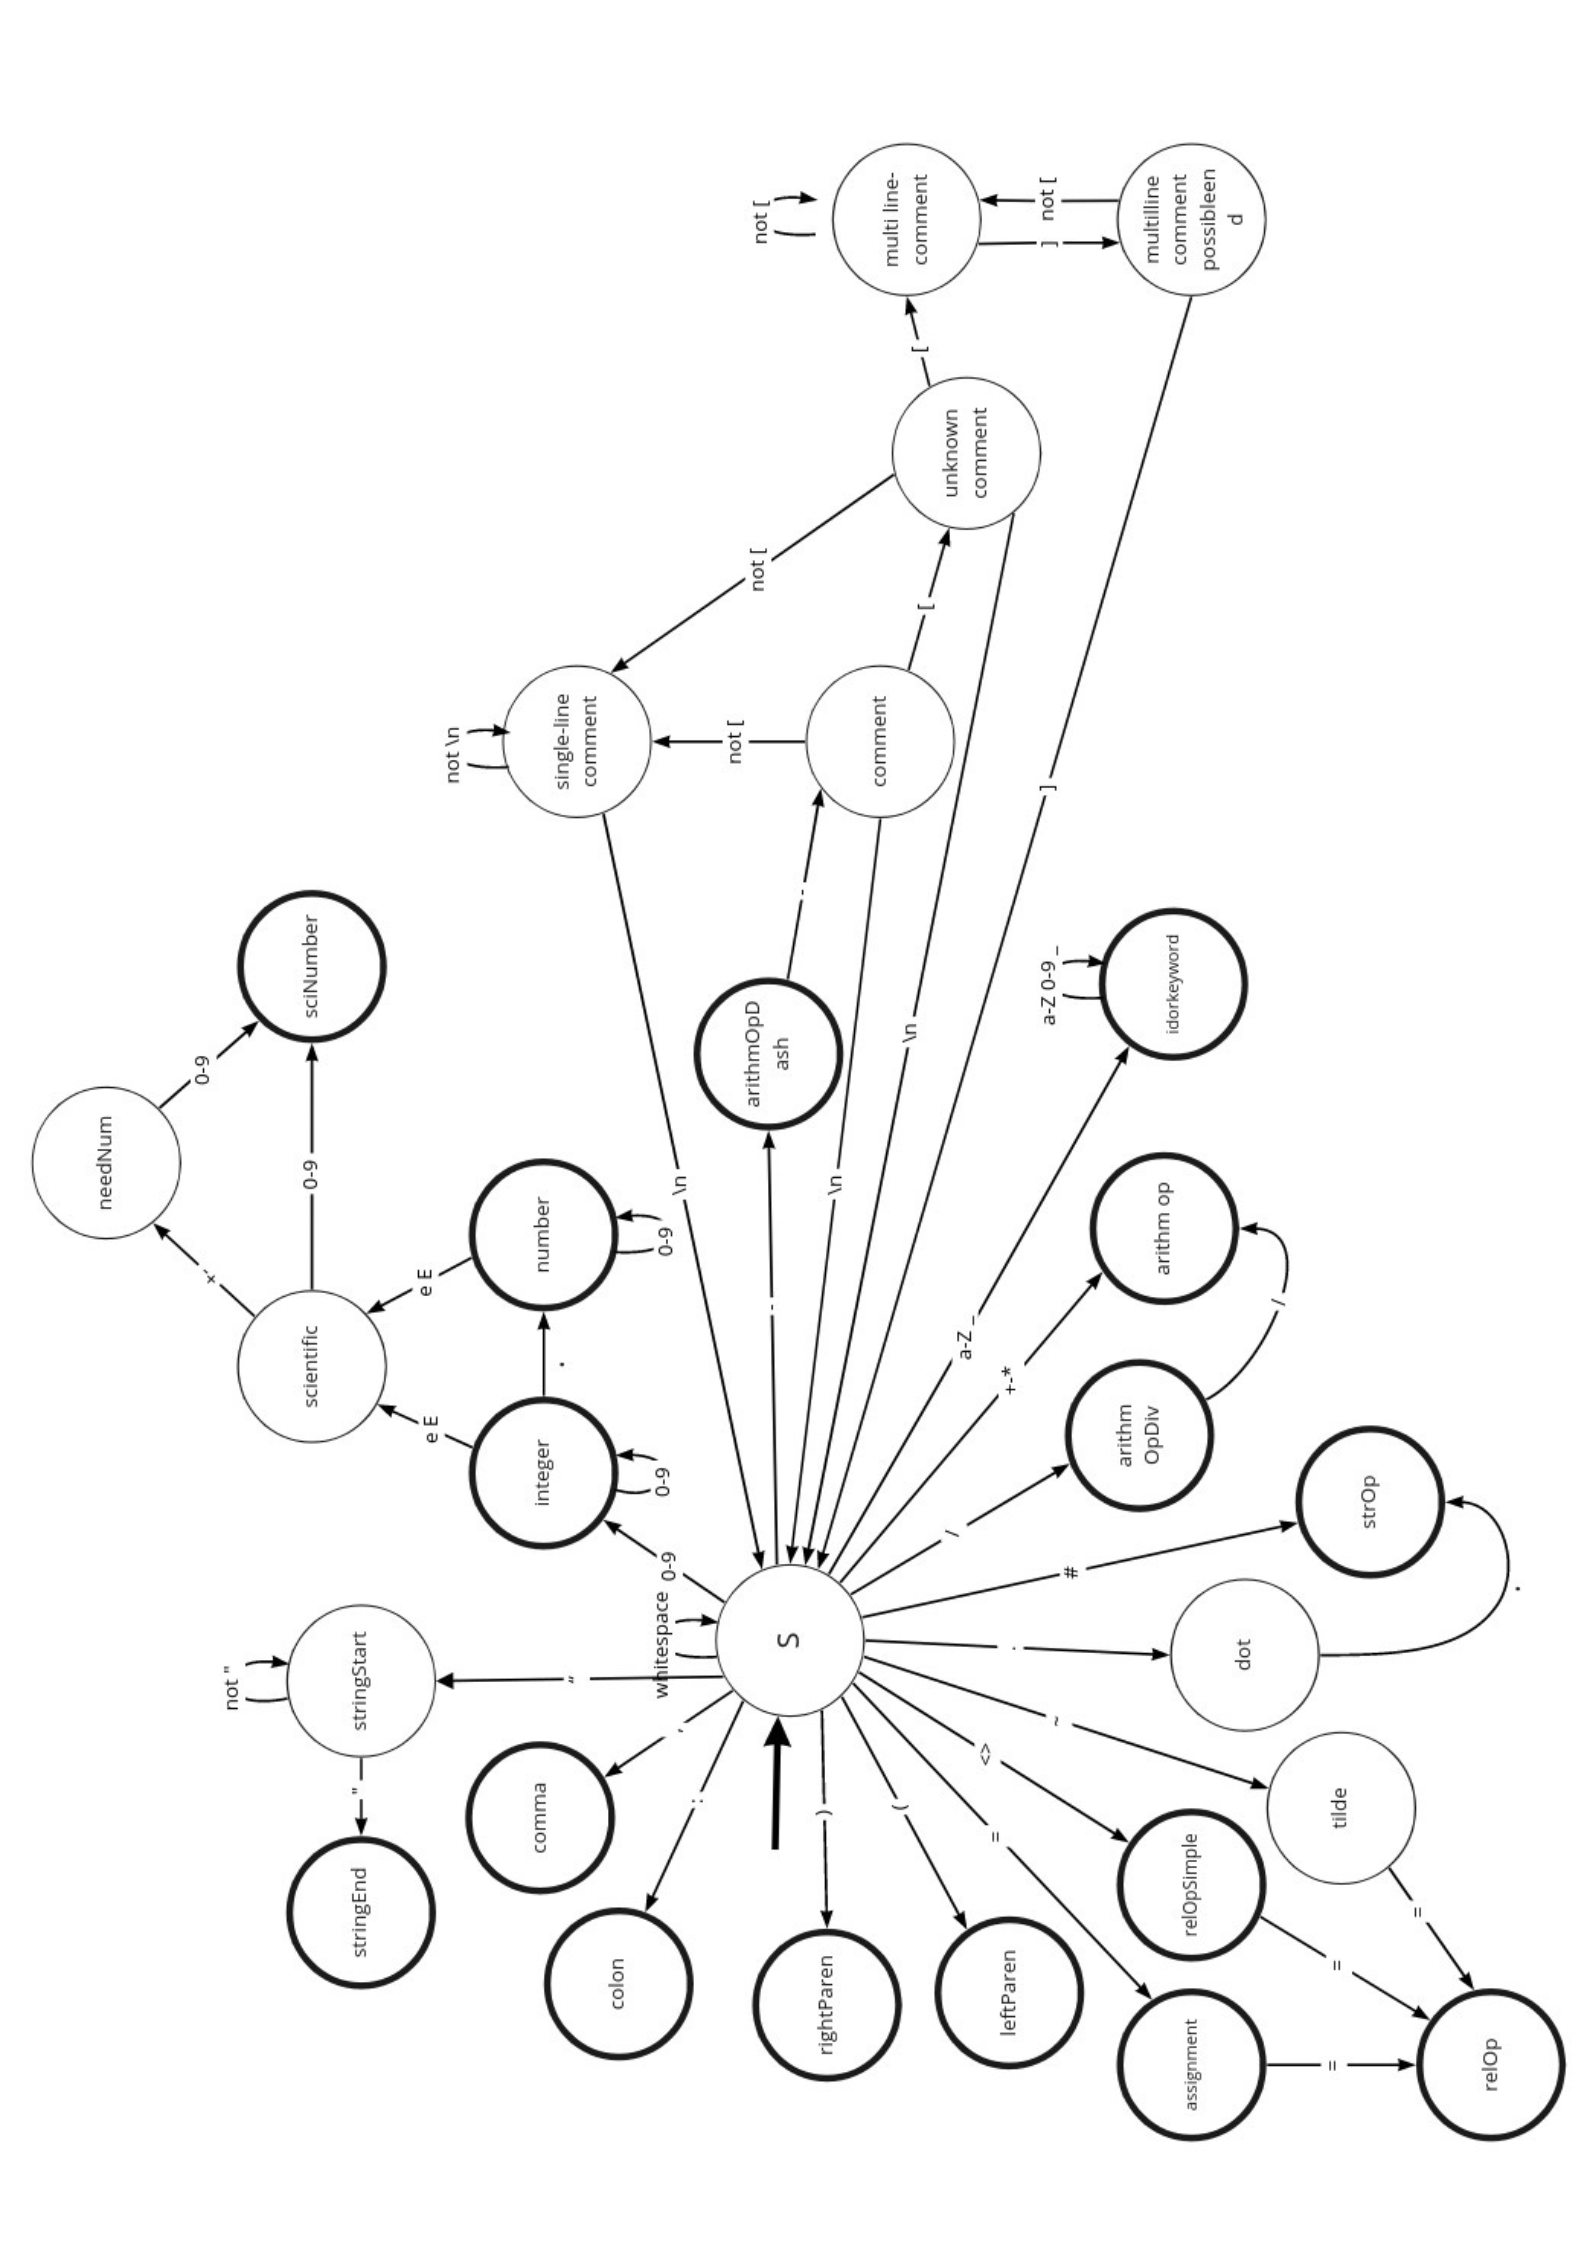
\includegraphics[scale=0.36]{fsm_rotated.png}

\end{document}
